%=====================================================================
%  Quantitative Reasoning - LAB 413
%  Lab 7: Confidence Intervals & Hypothesis Testing (Week 9 Recap)
%  Instructor: Subin Na
%  Beamer conversion of Lab7_1022_PPT.pptx
%  Compile: pdflatex Lab7_beamer.tex   (run twice for footline counters)
%=====================================================================
\documentclass[aspectratio=169,11pt]{beamer}

%---------------------------------------------------------------------
%  Packages
%---------------------------------------------------------------------
\usepackage[utf8]{inputenc}
\usepackage[T1]{fontenc}
\usepackage{lmodern}
\usepackage{amsmath,amssymb}
\usepackage{graphicx}
\usepackage{booktabs}
\usepackage{tcolorbox}
\tcbuselibrary{skins}

%---------------------------------------------------------------------
%  QR-Lab 413 theme  (shared across all 11 labs)
%---------------------------------------------------------------------
\usetheme{default}
\usecolortheme{default}
\useinnertheme{circles}

\definecolor{qrnavy}{RGB}{20,44,90}
\definecolor{qrblue}{RGB}{38,80,150}
\definecolor{qrgray}{RGB}{90,95,105}
\definecolor{qrlight}{RGB}{234,239,247}
\definecolor{qrred}{RGB}{190,60,60}

\setbeamercolor{structure}{fg=qrnavy}
\setbeamercolor{frametitle}{fg=white,bg=qrnavy}
\setbeamercolor{title}{fg=qrnavy}
\setbeamercolor{block title}{fg=white,bg=qrblue}
\setbeamercolor{block body}{bg=qrlight}
\setbeamercolor{itemize item}{fg=qrblue}
\setbeamercolor{itemize subitem}{fg=qrblue}
\setbeamerfont{frametitle}{series=\bfseries}
\setbeamertemplate{navigation symbols}{}

% Frametitle bar
\setbeamertemplate{frametitle}{%
  \nointerlineskip
  \begin{beamercolorbox}[wd=\paperwidth,ht=3.2ex,dp=1.2ex,leftskip=0.3cm]{frametitle}%
    \strut\insertframetitle\strut
  \end{beamercolorbox}%
}

% Footline: course | lab | slide number
\setbeamertemplate{footline}{%
  \leavevmode%
  \hbox{%
    \begin{beamercolorbox}[wd=.5\paperwidth,ht=2.4ex,dp=1ex,leftskip=.3cm]{author in head/foot}%
      \usebeamerfont{author in head/foot}\color{qrgray}\small Quantitative Reasoning -- LAB 413%
    \end{beamercolorbox}%
    \begin{beamercolorbox}[wd=.5\paperwidth,ht=2.4ex,dp=1ex,rightskip=.3cm]{title in head/foot}%
      \usebeamerfont{title in head/foot}\color{qrgray}\small\hfill Lab 7 \quad\insertframenumber\,/\,\inserttotalframenumber%
    \end{beamercolorbox}}%
}

% Handy "step number" badge (01, 02, ...) used on concept slides
\newcommand{\stepbadge}[1]{%
  \begin{tikzpicture}[baseline]\end{tikzpicture}%
}
\newtcbox{\numbadge}{on line,boxsep=2pt,left=4pt,right=4pt,top=2pt,bottom=2pt,
  colback=qrnavy,colframe=qrnavy,fontupper=\bfseries\color{white},arc=2pt}

% Key-concepts block
\newtcolorbox{keybox}[1][Key Concepts]{colback=qrlight,colframe=qrnavy,
  fonttitle=\bfseries,title={#1},coltitle=white,arc=2pt,left=4pt,right=4pt,
  top=3pt,bottom=3pt,boxrule=0.6pt}

%---------------------------------------------------------------------
%  Title data
%---------------------------------------------------------------------
\title{\bfseries Confidence Intervals \& Hypothesis Testing}
\subtitle{Week 9 Recap \textbullet\ Lab 7}
\author{Instructor: Subin Na}
\institute{Quantitative Reasoning -- LAB 413}
\date{October 22, 2025}

\begin{document}

%---------------------------------------------------------------------
%  Title slide
%---------------------------------------------------------------------
{\setbeamertemplate{footline}{}
\begin{frame}
  \vfill
  {\color{qrgray}\small Quantitative Reasoning -- LAB 413}\\[0.6em]
  {\usebeamerfont{title}\color{qrnavy}\huge\bfseries Confidence Intervals\\[0.15em]\& Hypothesis Testing\par}
  \vspace{0.4em}
  {\color{qrblue}\large Week 9 Recap \ \textbullet\ \ Lab 7}\par
  \vspace{1.6em}
  {\color{qrgray} Instructor: \textbf{Subin Na} \hfill October 22, 2025}
  \vfill
\end{frame}
}

%---------------------------------------------------------------------
%  Today's Plan
%---------------------------------------------------------------------
\begin{frame}{Today's Plan}
  \begin{columns}[T]
    \begin{column}{0.5\textwidth}
      \textbf{\color{qrnavy}1. Quick Recap}
      \begin{itemize}
        \item Overview
        \item Confidence Interval: Concept
        \item Confidence Interval: In Regression
        \item Hypothesis Testing: Logic
        \item One- vs.\ Two-Sided Tests
      \end{itemize}
    \end{column}
    \begin{column}{0.5\textwidth}
      \phantom{\textbf{x}}
      \begin{itemize}
        \item Interpreting Significance
        \item Statistical vs.\ Practical Significance
        \item Testing Errors
      \end{itemize}
      \vspace{0.8em}
      \textbf{\color{qrnavy}2. RStudio Practice}
    \end{column}
  \end{columns}
\end{frame}

%---------------------------------------------------------------------
%  01 Overview
%---------------------------------------------------------------------
\begin{frame}{\numbadge{01}\ \ Overview}
  \begin{itemize}
    \item \textbf{Goal:} Quantify the uncertainty behind point estimates using probability.
    \item Two types of statistical inference:
  \end{itemize}
  \vspace{0.6em}
  \begin{columns}[T]
    \begin{column}{0.48\textwidth}
      \begin{tcolorbox}[colback=white,colframe=qrnavy,arc=3pt,halign title=center,
        title=\bfseries Confidence Intervals,coltitle=white,colbacktitle=qrnavy]
        \centering estimate \textbf{population parameters}
      \end{tcolorbox}
    \end{column}
    \begin{column}{0.48\textwidth}
      \begin{tcolorbox}[colback=white,colframe=qrnavy,arc=3pt,halign title=center,
        title=\bfseries Hypothesis Tests,coltitle=white,colbacktitle=qrnavy]
        \centering assess \textbf{evidence about claims} concerning the population
      \end{tcolorbox}
    \end{column}
  \end{columns}
\end{frame}

%---------------------------------------------------------------------
%  02 CI concept
%---------------------------------------------------------------------
\begin{frame}{\numbadge{02}\ \ Confidence Intervals (1): Concept}
  \begin{keybox}
    \begin{itemize}
      \item A \textbf{point estimate} gives our best single guess of the population
            value (imperfect because of random sampling variability).
      \item A \textbf{confidence interval (CI)} provides a \emph{range of plausible
            values} for that population parameter.
    \end{itemize}
  \end{keybox}
  \vspace{0.5em}
  \begin{equation*}
    \text{CI} \;=\; \text{point estimate} \;\pm\; (\text{critical value}) \times (\text{standard error})
  \end{equation*}
\end{frame}

%---------------------------------------------------------------------
%  03 CI in regression
%---------------------------------------------------------------------
\begin{frame}{\numbadge{03}\ \ Confidence Intervals (2): In Regression}
  \begin{keybox}
    The CI shows how much \textbf{uncertainty} surrounds our estimated effect.
  \end{keybox}
  \vspace{0.6em}
  \textbf{\color{qrnavy}Example.} A one-month increase in age predicts a
  0.25-inch increase in height \quad(95\% CI: $0.22$--$0.28$).
  \vspace{0.6em}
  \begin{itemize}
    \item If we repeated this study many times, \textbf{95\% of the intervals}
          we compute would contain the true effect.
  \end{itemize}
\end{frame}

%---------------------------------------------------------------------
%  04 Hypothesis testing logic (1)
%---------------------------------------------------------------------
\begin{frame}{\numbadge{04}\ \ Hypothesis Testing: Logic (1)}
  \begin{keybox}
    Hypothesis testing is a \textbf{structured way to evaluate a claim} about a
    population parameter.
  \end{keybox}
  \vspace{0.8em}
  \begin{columns}[T]
    \begin{column}{0.5\textwidth}
      \begin{block}{Null hypothesis $H_0$}
        ``no effect'' or ``no difference''
      \end{block}
    \end{column}
    \begin{column}{0.5\textwidth}
      \begin{block}{Alternative hypothesis $H_1$}
        the effect or difference we want to detect
      \end{block}
    \end{column}
  \end{columns}
\end{frame}

%---------------------------------------------------------------------
%  05 Hypothesis testing logic (2) - steps
%---------------------------------------------------------------------
\begin{frame}{\numbadge{05}\ \ Hypothesis Testing: Logic (2)}
  \textbf{\color{qrnavy}Steps}
  \begin{enumerate}
    \item State $H_0$ and $H_1$.
    \item Collect data and calculate the test statistic ($z$).
    \item Compute the $p$-value $\rightarrow$ probability of observing such an
          extreme statistic if $H_0$ were true.
    \item Compare the $p$-value with $\alpha$ (e.g., $0.05$) $\rightarrow$ decide
          whether to reject $H_0$.
  \end{enumerate}
  \vspace{0.4em}
  \begin{center}
  \small
  $H_0,\,H_1 \;\longrightarrow\; \text{test statistic } z \;\longrightarrow\;
   p\text{-value} \;\longrightarrow\; \text{compare with }\alpha
   \;\longrightarrow\; \text{decision}$
  \end{center}
\end{frame}

%---------------------------------------------------------------------
%  06 One- vs two-sided  (EMBED normal-curve figure)
%---------------------------------------------------------------------
\begin{frame}{\numbadge{06}\ \ One- vs.\ Two-Sided Tests}
  \begin{keybox}
    The $p$-value depends on the type of alternative hypothesis.
    \begin{itemize}
      \item \textbf{One-sided:} tests for an effect in one direction (increase \emph{or} decrease only).
      \item \textbf{Two-sided:} tests for any difference; doubles the one-sided tail area.
    \end{itemize}
  \end{keybox}
  \vspace{0.3em}
  \begin{center}
    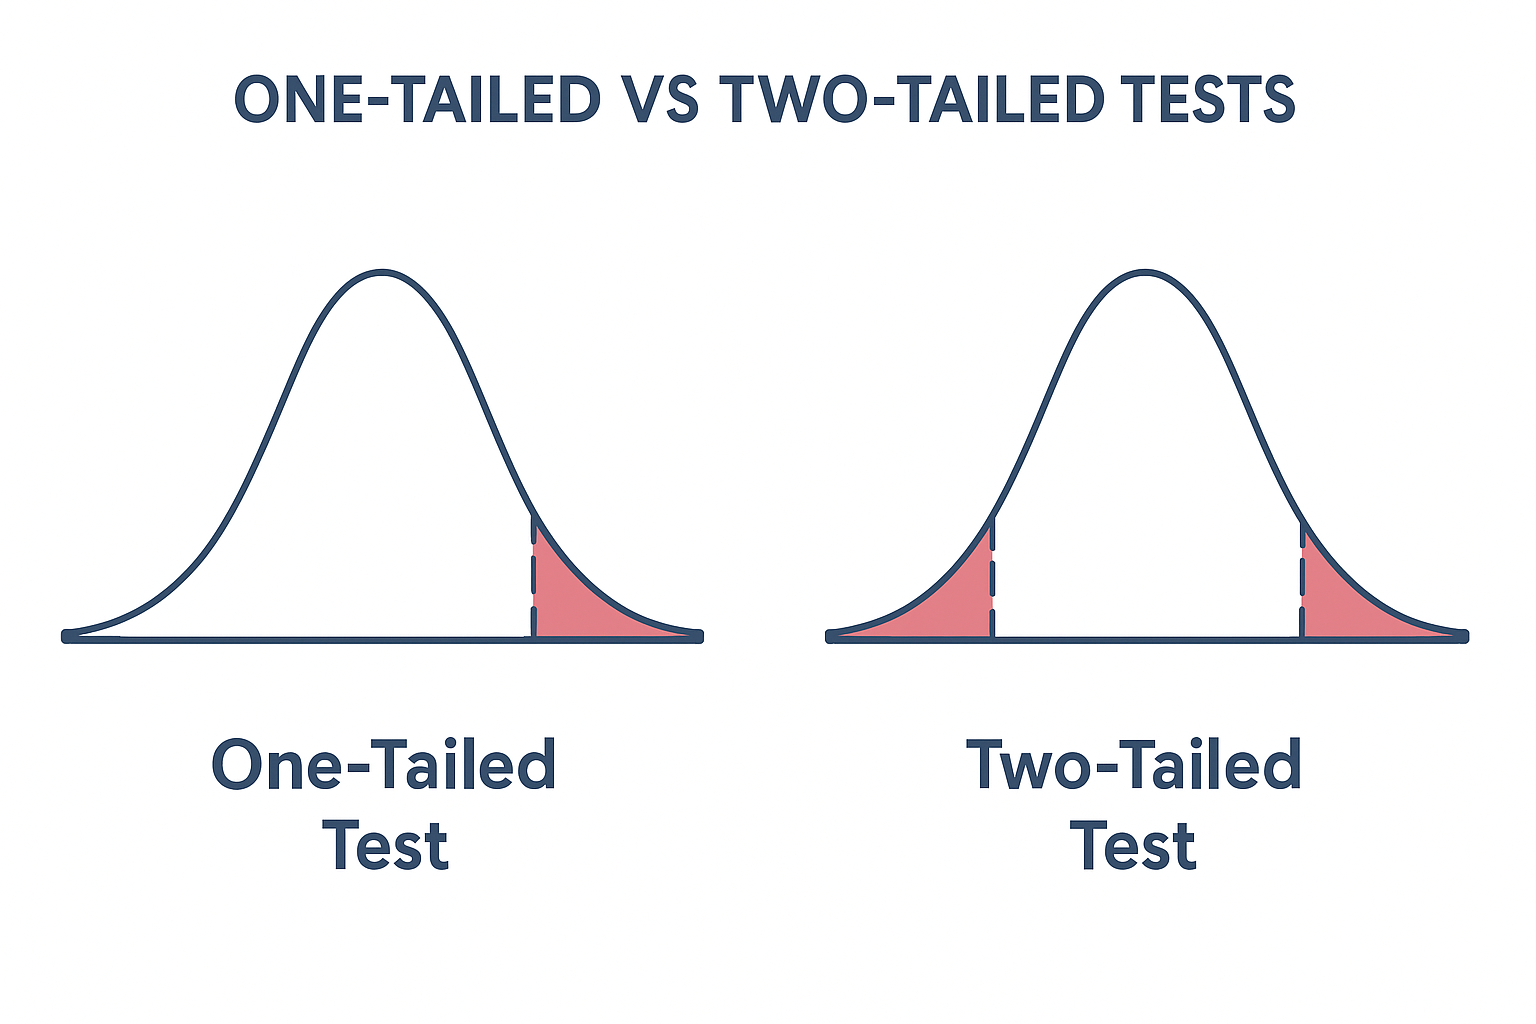
\includegraphics[width=0.72\textwidth]{figures/s08_1_6.9x3.0.png}
  \end{center}
\end{frame}

%---------------------------------------------------------------------
%  Worked example - setup
%---------------------------------------------------------------------
\begin{frame}{Worked Example: Coffee Consumption}
  \begin{keybox}[Scenario]
    A national survey reports adults drink an average of \textbf{2.8 cups} of
    coffee per day ($\sigma = 1.1$). You collect data from $n = 50$ Penn students
    and find they drink \textbf{3.2 cups} on average.
  \end{keybox}
  \vspace{0.6em}
  \begin{center}
    At $\alpha = 0.05$, is there evidence that Penn students drink
    \emph{more} coffee than the national average?
  \end{center}
\end{frame}

%---------------------------------------------------------------------
%  z-table (EMBED reference table)
%---------------------------------------------------------------------
\begin{frame}{Reference: Z-Score Table}
  \begin{center}
    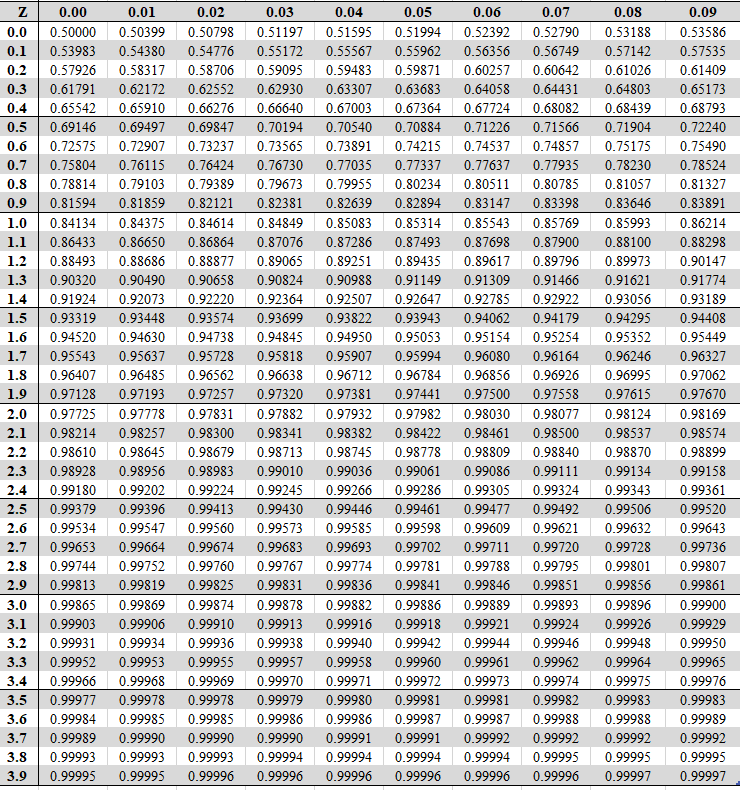
\includegraphics[height=0.74\textheight]{figures/s10_1_13.4x14.3.png}\\[0.3em]
    {\scriptsize\color{qrgray}Source: statisticsbyjim.com/hypothesis-testing/z-table/}
  \end{center}
\end{frame}

%---------------------------------------------------------------------
%  Worked example - solution
%---------------------------------------------------------------------
\begin{frame}{Worked Example: Solution}
  \small
  \begin{columns}[T]
    \begin{column}{0.44\textwidth}
      \textbf{\color{qrnavy}Given}
      \begin{align*}
        \mu_0 &= 2.8 \text{ cups/day}\\
        \bar{x} &= 3.2 \text{ cups/day}\\
        \sigma &= 1.1\\
        n &= 50\\
        \alpha &= 0.05
      \end{align*}
    \end{column}
    \begin{column}{0.56\textwidth}
      \textbf{\color{qrnavy}Test}
      \begin{align*}
        H_0&: \mu = 2.8 \quad(\text{No difference})\\
        H_1&: \mu > 2.8 \quad(\text{drink more})\\[0.4em]
        z &= \frac{\bar{x}-\mu_0}{\sigma/\sqrt{n}}
           = \frac{3.2-2.8}{1.1/\sqrt{50}} \approx 2.57
      \end{align*}
      \vspace{0.2em}
      \begin{tcolorbox}[colback=qrlight,colframe=qrred,arc=2pt,boxrule=0.6pt]
        $p = 0.0051 < 0.05 \;\Rightarrow\; \textbf{Reject } H_0$\\
        Strong evidence Penn students drink more coffee than the national average.
      \end{tcolorbox}
    \end{column}
  \end{columns}
\end{frame}

%---------------------------------------------------------------------
%  07 Interpreting significance
%---------------------------------------------------------------------
\begin{frame}{\numbadge{07}\ \ Interpreting Significance}
  \begin{keybox}
    \begin{itemize}
      \item A ``significant'' result means our data are \emph{unlikely} if $H_0$
            were true --- \textbf{not} that the effect is large or important.
      \item Report exact $p$-values \textbf{and} effect sizes, not just
            ``significant'' vs.\ ``not significant.''
    \end{itemize}
  \end{keybox}
  \vspace{0.5em}
  \begin{tcolorbox}[colback=white,colframe=qrblue,arc=2pt]
    Students drank an average of \textbf{3.2} cups/day, compared to the national
    mean of \textbf{2.8} \\(mean difference $= 0.4$ cups, $p = 0.005$,
    95\% CI $[0.13,\,0.67]$).
  \end{tcolorbox}
\end{frame}

%---------------------------------------------------------------------
%  08 Statistical vs practical significance
%---------------------------------------------------------------------
\begin{frame}{\numbadge{08}\ \ Statistical vs.\ Practical Significance}
  \begin{itemize}
    \item \textbf{Statistical significance:} result unlikely due to chance ($p < \alpha$).
    \item \textbf{Practical significance:} result is large or meaningful in context.
    \item \textbf{Causal significance:} result can be interpreted causally
          (requires experimental / randomized design).
  \end{itemize}
  \vspace{0.6em}
  \begin{center}
  \renewcommand{\arraystretch}{1.3}
  \begin{tabular}{@{}lll@{}}
    \toprule
    \textbf{Type} & \textbf{Example} & \textbf{Interpretation}\\
    \midrule
    Statistical & $p = 0.03$ & Evidence against $H_0$\\
    Practical   & Effect $= 0.01$ vs.\ $2.0$ & Magnitude matters\\
    Causal      & RCT effect & Can infer causality\\
    \bottomrule
  \end{tabular}
  \end{center}
\end{frame}

%---------------------------------------------------------------------
%  09 Testing errors
%---------------------------------------------------------------------
\begin{frame}{\numbadge{09}\ \ Testing Errors}
  \begin{keybox}
    \begin{itemize}
      \item \textbf{Type I Error ($\alpha$):} rejecting a \emph{true} null hypothesis (false positive).
      \item \textbf{Type II Error ($\beta$):} failing to reject a \emph{false} null hypothesis (false negative).
      \item \textbf{Power ($1-\beta$):} probability of correctly rejecting a false null.
    \end{itemize}
  \end{keybox}
  \vspace{0.5em}
  \begin{center}
    High power $\Rightarrow$ a good chance of detecting an effect when it truly exists.
  \end{center}
\end{frame}

%---------------------------------------------------------------------
%  Transition to RStudio
%---------------------------------------------------------------------
{\setbeamertemplate{footline}{}
\begin{frame}
  \vfill
  \centering
  {\color{qrnavy}\Huge\bfseries RStudio Practice}\\[0.8em]
  {\color{qrblue}\large Confidence Intervals \& One-Sample $t$-test}\\[0.4em]
  {\color{qrgray} See \texttt{Lab7.Rmd} / \texttt{Lab7\_1022.R}}
  \vfill
\end{frame}
}

\end{document}
